\documentclass[sigconf, anonymous]{acmart}

\usepackage{booktabs} % For formal tables

%\usepackage{arev}
\usepackage{listings}
\usepackage{caption}
\usepackage{booktabs}
\usepackage{rotating}
\usepackage{subcaption}
\usepackage{amsmath}
\usepackage{color}
\usepackage{tikz}
\usepackage{amsfonts}
\usepackage{amssymb}
\usepackage[noend]{algpseudocode}
\usepackage{algorithm,float}
\usepackage{array}
\usepackage{enumitem}
\usetikzlibrary {shapes.geometric,positioning,arrows,shadows}
\usetikzlibrary{decorations.pathreplacing}
\definecolor{myBlue}{RGB}{0,162,227}
\definecolor{apricot}{RGB}{251,185,130}
\renewcommand{\theoremautorefname}{Definition}


 
\newcommand*\circled[1]{\tikz[baseline=(char.base)]{
            \node[shape=circle,draw,inner sep=2pt] (char) {#1};}}

\newcommand{\todo}[1]{\textcolor{red}{TODO: #1}}


% Copyright
%\setcopyright{none}
%\setcopyright{acmcopyright}
%\setcopyright{acmlicensed}
\setcopyright{rightsretained}
%\setcopyright{usgov}
%\setcopyright{usgovmixed}
%\setcopyright{cagov}
%\setcopyright{cagovmixed}



% DOI
%\acmDOI{10.475/123_4}

% ISBN
%\acmISBN{123-4567-24-567/08/06}

%Conference
%\acmConference[WOODSTOCK'97]{ACM Woodstock conference}{July 1997}{El
%  Paso, Texas USA} 
%\acmYear{1997}
%\copyrightyear{2016}
%
%\acmPrice{15.00}

%\title: Think Outside the Box: Exploring and Exploiting Cross-Language Optimizations in SCOPE
\newcommand{\nonNativeTimeL}{43.70}
\newcommand{\nonNativeTimeU}{73.32}
\newcommand{\optimizableU}{0.16}
\newcommand{\potentiallyOptimizableU}{6.76}
\newcommand{\potentiallyOptimizableL}{1.01}




\begin{document}
\title{Exploring Cross-Language Optimizations in Big Data Systems: An Empirical Study of SCOPE}
%\titlenote{Produces the permission block, and
%  copyright information}
%\subtitlenote{The full version of the author's guide is available as
%  \texttt{acmart.pdf} document}


\author{Marija Selakovic}

%\orcid{1234-5678-9012}
\affiliation{%
  \institution{TU Darmstadt}
  \state{Germany} 
}
\email{m.selakovic89@gmail.com}

\author{Michael Barnett}

\affiliation{%
  \institution{Microsoft Research}
  \state{USA} 
}
\email{Michael.Barnett@microsoft.com}

\author{Madan Musuvathi}

\affiliation{%
  \institution{Microsoft Research}
    \state{USA} 
    }

  
\email{madanm@microsoft.com}



\author{Todd Mytkowicz}

\affiliation{%
  \institution{Microsoft Research}
    \state{USA} 
    }

  
\email{toddm@microsoft.com}


% The default list of authors is too long for headers}
\renewcommand{\shortauthors}{M. Selakovic et al.}


\begin{abstract}

  Building scalable big data programs currently requires programmers to combine relational (SQL) with non-relational code (Java, C$\sharp$, Scala).
  Relational code is declarative --- a program describes \emph{what} the computation is and the compiler decides \emph{how} how to distribute the program.  SQL query optimization has enjoyed a rich and fruitful history, however, most research and commercial optimization engines treat non-relational code as a black-box and thus are unable to optimize it.

  This paper empirically studies over 3 million SCOPE programs across five data centers within Microsoft and finds programs with non-relational code take between 45-70\% of data center CPU time. We further explore the potential for SCOPE optimization by generating more native code from the non-relational part. Finally, we present 5 case studies showing that triggering more generation of native code in these jobs yields significant performance improvement: optimizing just one portion resulted in as much as 25\% improvement for an entire program.

\end{abstract}

%
% The code below should be generated by the tool at
% http://dl.acm.org/ccs.cfm
% Please copy and paste the code instead of the example below. 
%



%\keywords{ACM proceedings, \LaTeX, text tagging}


\maketitle

\section{Introduction}
Large-scale data-processing frameworks, such as MapReduce~\cite{MapReduce}, SCOPE~\cite{SCOPE}, Hadoop~\cite{Hadoop}, Spark~\cite{Spark}, have become an integral part of computing today. One reason for their immense popularity is that they provide a simplified programming model that greatly simplifies the distribution and fault-tolerance of big-data processing. For instance, frameworks like SCOPE and Spark provide a SQL-like declarative interface for specifying the relational skeleton of data-processing jobs while providing extensibility by supporting expressions and functions written in general-purpose languages like C\#, Java, or Scala. 

%\emph{MapReduce} framework has become an immensely popular for easy development of scalable parallel applications that process large amounts of data. 
%The advantage of MapReduce is that it isolates the details of running a big data application as a distributed program. 
%To ease the use of MapReduce, several projects (Apache Pig, Apache Hive or SCOPE) provide high-level declarative interfaces on top of the MapReduce framework. 
%This means that big data processing jobs are composed of queries expressed in an SQL-like declarative language with expressions written in languages like Java, C\# or Scala.
The relational aspect is crucial: it is what enables the automatic parallelization for efficiently scaling out to arbitrary amounts of data.
Big data systems assume that the non-relational part is written carefully enough so that it does not violate the assumptions needed for automatic parallelization: i.e., programmers must write their non-relational logic to be deterministic and insensitive to the ordering of the input.

However, these systems are known to lag far behind traditional database systems in runtime efficiency~\cite{Jahani:2011,Pavlo:2009}, primarily because of the flexibility of the programming model they support. For instance,  a key bottleneck in Spark is neither the disk nor the network, but the time spent by the CPU on compression/decompression of data, serialization/deserialization of the input into/from Java objects, and the JVM garbage collection~\cite{ousterhout-nsdi15}. SCOPE,  described more fully in Section~\ref{sec:Scope}, supports a hybrid native (C++) and C\# runtime partly to alleviate this overhead.
Like SCOPE, Hadoop Streaming lets programmers write programs in a mix of languages\cite{hadoop_stream}. 
Our analysis shows that this cross-language interaction (in SCOPE, between the native and C\# runtimes) is a significant cost in the overall system.  
Equally importantly, the presence of non-relational code blocks the powerful relational optimizations implemented in these data-processing runtimes~\cite{non-relational-opt-papers}. 


The goal of this work is to study and better understand the key performance bottlenecks in modern data-processing systems, and demonstrate the potential for cross-language optimizations. While this paper is primarily about SCOPE, we believe our results and optimizations generalize to other data-processing systems. 
%SCOPE (Structured Computations for Parallel Execution) is a query language that combines relational logic written in SQL with user expressions written in C\#.
SCOPE is the key data-processing system used at Microsoft running at least half a million jobs daily on serveral Microsoft data centers. 
Figure~\ref{fig:example} shows a simple example of a SCOPE program (hereafter referred to as a {\em script}) that interleaves relational logic with C\# expressions.

%To achieve this goal, we empiricaly analyse over 3,000,000 SCOPE jobs that run across five data centers at Microsoft during one week. 

%The language supports MapReduce programming model and is developed at Microsoft for big data processing. 
%Nowadays, it is used for almost 450,000 daily jobs running on several data centers in Microsoft.


%One source of inefficiency is due to non-relational code found in big data queries. 
%Despite powerfulness of SQL optimizations, such optimizations can not be applied to arbitrary code written in an imperative language.
%This calls for cross language optimizations in order to obtain a high-level efficiency of processing big data jobs.
%Moreover, we believe that increasing hardware and computing power is no longer a sustainable way of improving the efficiency of big data processing . 

%The goal of this work is to understand how the time is spent in big-data jobs and where is a potential for cross language optimizations.

%As described later in Section~\ref{sec:background}, the stage of SCOPE job can run as native (C++) if it does not contain any non-relational code. 
%However, this is unlikely the case and to run C\# code in SCOPE script the runtime performs data serialization from C++ format to format required by .NET runtime. 
%This process of data serialization and deserialization is inherently very expensive and to increase the number of job stages that run as native, the SCOPE compiler provides C++ implementation for a subset of .NET framework methods. 
%To illustrate when SCOPE script runs as native vs. non-native, consider examples in Figure~\ref{fig:example}. 
%Both code fragments are very simple SCOPE jobs. 
%The script in Figure~\ref{fig:native} runs as native, because SCOPE compiler has C++ implementation for \emph{String.isNullOrEmpty} method. On the other hand, the script in Figure~\ref{fig:non-native} has a call to \emph{Split} method, which is not optimized by the compiler and this causes entire script to run as non-native (C\# code).

\begin{figure}[ht]
 \begin{minipage}[b]{\linewidth}
  
   \begin{verbatim}
data = SELECT *
  FROM inputStream
  WHERE !String.IsNullOrEmpty(A) AND B == "Key1";
\end{verbatim}

    \subcaption{Predicate visible to optimizer.}
    \label{fig:native}
  \end{minipage}
  %
  \begin{minipage}[b]{\linewidth}
   \begin{verbatim}
data = SELECT *
  FROM inputStream
  WHERE M(A, B);

#CS
bool M(string x, string y) {
   return !String.IsNullOrEmpty(x) && y == "Key1";
}
#ENDCS
    \end{verbatim}

    \subcaption{Predicate invisible to optimizer.}
    \label{fig:non-native}
  \end{minipage}


\caption{Script Examples}
\label{fig:example}
\end{figure}

In Figure~\ref{fig:native}, the predicate in the {\tt WHERE} clause is subject to two potential optimizations:
\begin{enumerate}
\item The optimizer may choose to {\em promote} one (or both) of the conjuncts to an earlier part of the program, especially if either {\tt A} or {\tt B} are columns used for partitioning the data.
This can dramatically reduce the amount of data needed to be transferred from one vertex to another.
\item The SCOPE compiler has a set of methods that it considers to be {\em intrinsics}.
An intrinsic is a .NET method for which the SCOPE runtime has a semantically equivalent native function.
For instance, the method {\tt String.isNullOrEmpty} checks whether its argument is either null or else the empty string.
The corresponding native method is able to execute on the native data encoding which does not involve creating any .NET objects or instantiating the .NET virtual machine (CLR).
\end{enumerate}

On the other hand, Figure~\ref{fig:non-native} shows a slight variation where the user implemented the predicate in a separate C\# method. Unfortunately, the SCOPE compiler treats the call to user-defined functions as a black box. As a result, both optimizations are disabled and the predicate is executed in a C\# virtual machine. The resulting serialization and data-copying costs can reduce the throughput of the job by as much as XXX percent. 


%has a call to \emph{Split} method, which the SCOPE compiler does not understand. This causes the ent


%which is not optimized by the compiler and this causes entire script to run as non-native (C\# code).

When facing a performance regression, a performance analyst first measures her system to understand where the bottlenecks are.  Then, she can act on those data to make her system faster.  While such an approach is well understood and easy to execute for desktop software, it becomes challenging in the context of a massive distributed system, like SCOPE.
This paper first describes \emph{how} we built a datacenter-wide profiler so we could even start to measure application bottlenecks.
Our new profiling infrastructure is a combination of offline static analysis of the executed code in addition to low-overhead online measurements captured by SCOPE's runtime.
Then, the paper describes the results of our profiling of over 3 million SCOPE programs across five data centers within Microsoft.
We find programs with non-relational code take between 45-70\% of data center CPU time.  

% %Despite knowing the cause of inefficiencies, still the little is known about how much time SCOPE jobs spend in non-relational code and what are the opportunities to trigger more generation of native code. 
% To answer these questions, we propose a new profiling infrastructure based on static analysis of job artifacts.
% By doing this, we are able to post-analyse large amount of jobs without introducing any additional overhead.
% Except the time spent in non-relational code, our profiling approach also surveys different sources of non-relational code in SCOPE jobs.
% It returns a list of most commonly used framework methods, for which having C++ implementation would trigger more generation of native code.
Finally, we discuss the effects of cross-language optimization based on \emph{method inlining}. 
The idea behind method inlining is to instead calling a method, move the logic of that method to the operator. By doing this, the compiler is able generate native code from inlined logic.
We prove the effectiveness of such optimizations in Z case studies by optimizing K jobs from U different teams at Microsoft. 

% Our experimental evaluation shows that non-native code takes between 45-75\% of data center CPU time. By further increasing the list of framework functions that have native implementation we can optimize up to Z\% of data center time.
% Finally, we illustrate that performance impact of inlining jobs to run as native is statistically significant and range between A and B\%. 

% As a consequence, our findings motivate future research in at least two ways.
% First, on tools and techniques that help developers write more efficient big data jobs by avoiding unnecessary generation of non-native code. 
% Second, on compiler optimizations that automatically generate native code from the non-relational logic.


% In summary, this work contributes the following:
% \begin{itemize}
% \item \emph{Profiling infrastructure for analyzing SCOPE jobs.} 
% We present the approach for profiling data centers based on static analysis of job artifacts. 
% The approach reports time spent in relational vs non-relational code and detects different sources of non-relational code for every jobs stage. 

% \item \emph{Reporting opporunities for cross-language optimizations.} We discuss two possible ways to enable further generation of native code. 
% First, we survey the most relevant framework functions relevant for native implementation. 
% Second, we present an analysis to find opportunities that trigger the generation of native code by \emph{inlining} user-written functions.  

% \item \emph{Empirical evidence.} 
% We illustrate by X case studies that enabling job stage to run as native code signifcantly improve the job performance by factors Y-K.
% \end{itemize}



\section{Background}
\label{sec:background}
Many (all?) ``Big Data" systems are actually a mixture of languages \cite{}.
In general, we categorize them as comprising a {\it relational} part and a {\it non-relational} part.
The former is some variant of SQL \cite{}, i.e., a declarative data-flow language that expresses how data flows
from inputs to outputs (both usually being relational tables) through a series of data-parallel operators
such as filters, projections, and various types of joins.
The non-relational part is expressed in an imperative language, like C\#, Java, Scala, or Python \cite{}.

The relational aspect is crucial: it is what enables the automatic parallelization for efficiently scaling out to
arbitrary amounts o data.
Big data systems often assume that the non-relational part was written carefully enough so that it does not
violate these assumptions: i.e., programmers must write their non-relational logic to be deterministic and insensitive
to the ordering of the input.

\subsection{Scope Language}
SCOPE \cite{} is a Big Data system used internally within Microsoft.
However it is transitioning into an external offering as U-SQL \cite{}.
Its relational part is very similar to SQL, enough so that we will ignore any differences.
The non-relational part is C\#\cite{}.
This means that all expressions in a SCOPE program (aka {\it script}) are written as C\# expressions.
In addition, SCOPE allows user-defined functions (written as C\# methods) and user-defined operators
(written as C\# classes).

\subsubsection{Execution of a Scope Script}
A SCOPE script defines a directed acyclic graph (DAG) where each vertex is a set of operators implemented on the
same physical (or virtual) machine. We use the term {\it node} for the physical or virtual machine that a
vertex is implemented on.
The edges of the DAG are communication channels that use a high-speed communication network between nodes.
The operators within a vertex are the end product of a very sophisticated optimizer \cite{}; expressions written
within a certain construct in the script may end up being executed in vertices that do not correspond to the
construct in a simple manner.
For instance, a sub-expression from a filter may be {\it promoted} into a vertex which extracts an input
table from a data source, whereas the rest of the filter may be in a vertex that is many edges distant from
the input layer.

\subsection{Running C++ vs. C\# Vertex}
The SCOPE compiler generates both C++ and C\# operators for the same source-level construct.
Each operator, however, must execute either entirely in C\# or C++: mixed code is not provided for.
Thus, when possible, the C++ operator is preferred because the data layout in stored data uses C++ data structures.
Thus, for example, a simple projection of a subset of the columns can be done entirely
without using the .NET Runtime.
But when a script contains a C\# expression, such as in Figure~\ref{example:SimpleFilter}, then
each row in the input table must be converted to a C\# representation, i.e., a C\# object representing
the row must be created.
Then the C\# expression can be evaluated in the .NET Runtime.

Because this can be inefficient, the SCOPE runtime contains C++ functions that are semantically
equivalent to a subset of the .NET Framework methods that are frequently used; these are called
{\it intrinsics}.
The SCOPE compiler then emit calls to the (C++) intrinsics in the C++ generated operator, which is
then used at runtime in preference to the C\# generated operator.
(As opposed to using {\it interop} to execute native code from within the .NET Runtime.)



\section{Profiling Infrastructure for Data Centers}
Jobs run on a distributed computing platform, called Cosmos, designed for storing and analyzing massive data sets. Cosmos runs on five clusters consisting of thousands of commodity servers~\cite{SCOPE}. Cosmos is highly scalable and performant: it stores exabytes of data across hundreds of thousands of physical machines. Cosmos runs millions of big-data jobs every week and almost half million jobs every day. It is used by more than 10,000 developers at Microsoft running very diverse workloads and scenarios.

Finding optimization opportunities that are applicable to such a large number of diverse jobs is a very challenging problem.
We can hope to find interesting conclusions only if our profiling infrastructure is scalable. To achieve this, the important aspect to consider is \emph{what type of information we should analyze}. In the following sections, we describe our major decisions when building infrastructure for profiling big data jobs.

\subsection{Job Artifacts}
\label{sec:artifacts}

After execution of a SCOPE job finishes, the runtime produces several artifacts that contain code and runtime information for every job stage.
Job artifacts are indefinitely stored within Cosmos itself in a {\em job repository}.
This provides two benefits: we can derive data for a relatively large number of jobs since we do not require re-running them, and we can also answer more complex, but interesting questions, such as which job stages run as C++ vs. C\#.
We provide an overview of the subset of artifacts which we use to profile the data center.

\paragraph{Job Algebra}

The job algebra is a graph representation of the job execution plan. Job vertices are presented as outer-most nodes in a graph. Each job vertex contains all operators that run inside that vertex and an operator can be either user-defined or native. Optionally, if all operators are native, the vertex can be marked with the \emph{nativeOnly} flag, indicating that the entire vertex runs as native (C++). However, it does not distinguish between native and user-defined operators.


\paragraph{Runtime Statistics}
The runtime statistics file provides information on execution time for every job vertex and every operator inside the vertex. Among other statistics it includes CPU times, which we use as the primary metric of performance.
{\bf mb:[Should we cite that paper which says that many big data programs are cpu bound?]}

%\paragraph{Binaries}
%The job repository stores a job and all third-party projects in binary format (dll) that contains both native and managed code (.NET) with the generated assembly code.


\paragraph{Generated C\# and C++ Code}
The SCOPE compiler generates both C\# and C++ code for every job.
An artifact containing the C++ code has for every vertex a code region containing a C++ implementation of the vertex and another code region that provides class names for every operator that runs as C\#.
An artifact containing the C\# code includes implementations of non-native operators and user-written classes and functions defined inside the script.
Both source and binary are available for the generated code.

\subsection{Static Analysis}

After collecting the artifacts described in Section~\ref{sec:artifacts}, we perfom static analysis to detect different sources of C\# code in every vertex of a job. This is important to understand the opportunities for optimizing job vertices through C\# to C++ translation. For instance, a vertex can run as managed code due to only a single method call, or because of more complex C\# code.

Figure~\ref{fig:analysis} gives an overview of our analysis. It has two main components: \emph{Analysis of C++ code} and \emph{Analysis of C\# code}. Each analysis performs on the granularity of a job vertex. The goal is to look for opportunities to run an entire vertex as C++ code, which would remove all steps of data serialization between user and native operators within the vertex.


\begin{figure}[ht]
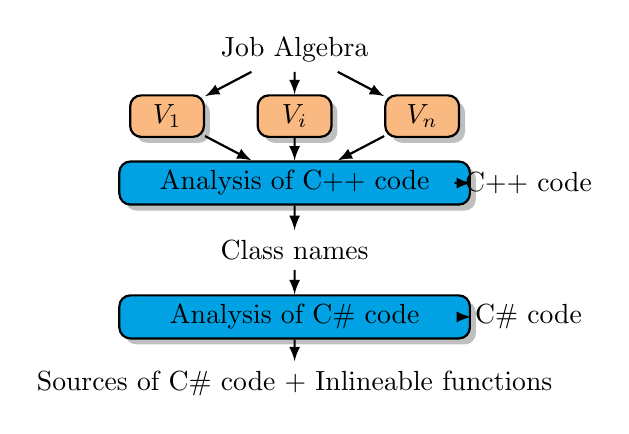
\begin{tikzpicture}[>=latex,xscale=2.7,yscale=.85,text centered,line 
  width=.8pt]
\tikzstyle{every node}=[draw,rounded corners,drop 
shadow,minimum height=1em]
\draw (1.1, 8) node[draw,text width=2em, fill = apricot] (vi) {$V_{i}$};
\draw (0.5,8) node[draw,text width=2em, fill = apricot] (vone) {$V_{1}$};
\draw (1.7,8) node[draw,text width=2em, fill = apricot] (vn) {$V_{n}$};
\draw (1.1,7) node[draw,text width=12em, fill = myBlue] (cplus) {Analysis of C++ code};
\draw (1.1,5) node[draw,text width=12em, fill = myBlue] (cs) {Analysis of C\# code};





\tikzstyle{every node}=[]
\draw (1.1,9) node[] (alg) {Job Algebra};
\draw (2.2,7) node[] (cpluscode) {C++ code};

\draw (1.1,6) node[] (names) {Class names};
\draw (2.2,5) node[] (cscode) {C\# code};
\draw (1.1,4) node (src) {Sources of C\# code + Inlineable functions};


\draw[->] (alg) -- (vi);
\draw[->] (alg) -- (vone);
\draw[->] (alg) -- (vn);
\draw[->] (vi) -- (cplus);
\draw[->] (vone) -- (cplus);
\draw[->] (vn) -- (cplus);
\draw[->] (cplus) -- (names);
\draw[->] (names) -- (cs);
\draw[->] (cs) -- (src);
\draw[->] (cpluscode) -- (cplus);
\draw[->] (cscode) -- (cs);

\end{tikzpicture}


\caption{High level picture of static analysis}
\label{fig:analysis}
\end{figure}

The first step of the analysis is to extract names of every job vertex, which serve as unique identifiers for vertices. Then for each vertex, the analysis parses generated C++ to find the class containing the vertex implementation. As discussed in Section~\ref{sec:artifacts}, for each vertex, C++ implementation contains two code regions: one that indicates which part of a vertex runs as C++ code and another region listing class names of operators that run as C\# code. If the latter region is empty, we conclude that entire vertex runs as C++ code. The output of the first stage of our analysis is the collection of class names that contain C\# operators.

Based on the output of the previous stage, the analysis parses generated C\# code to find definitions and implementation of every class in the list. The implementation of managed operators contains two sources of C\# code: generated code, which we whitelist and skip in our analysis and the user-written code. After analyzing user code, the analysis outputs the following sources of method calls:
\begin{itemize}
\item .NET framework calls
\item User written functions
\item User written operators 
\end{itemize}

We are particularly interested in the first two categories. It is not unusual case when a vertex runs as C\# execution just because of a framework method. We want to know what are the most important framework methods to optimize to enable C++ translation for a large number of vertices. Furthermore, we observe the cases when a logic of user-written function is relatively simple, and inlining the function logic as demonstrated in Figure~\ref{fig:example} would enable generation of C++ instead of C\# code. 

The details on how we detect different sources of managed code and inlineable functions are described as follows.

\subsubsection{Detecting Sources of C\# Code}
To find .NET framework calls, it is enough to check whether a method definition comes from .NET runtime. The analysis finds user-written functions by looking for their definition inside the script or in third-party projects. Because Cosmos repository keeps only binaries of third-party projects, we further analyze only user functions for which the source code is available. It is easier to optimize these functions through inlining (as described in Section~\ref{sec:analysisUser}), because we can manually confirm the correctness of inlined code. Finally, in SCOPE, users can easily implement their own operators: extractors (for parsing and constructing rows from a file), processors and reducers (for row processing), and combiners (for processing rows from two input tables). The analysis finds user operators by checking the interface the class implements. We do not consider user operators for C++ translation: they generate quite complex code which would be non-trivial to translate into C++.


\subsubsection{Analysis of User-Written Code}
\label{sec:analysisUser}
Inlining of a user-written function refers to moving a logic of the function to the script operator. We define \emph{inlineable} methods as follows.
\begin{definition}[Inlineable method]
Method $m$ is \emph{inlineable} if it has the following properties:
\begin{itemize}
\item It contains only .NET framework calls
\item It does not contain loops and try-catch blocks
\item It does not contain any assignment statements.
\item It does not contain any references to the fields of an object.
\item For all calls inside the method, arguments are passed by value (i.e., no {\em out} parameters or call-by-reference parameters).
\end{itemize}


\end{definition}

Furthermore, we distinguish among inlineable methods those that allow for \emph{instant} C++ generation, because all called .NET framework methods are \emph{intrinsics}. However, the analysis of other inlineable functions is important, because it provides the intuition on how many vertices are potentially optimizable in this way.

%We only consider for inlineing the methods defined inside the script, because their source code is available. Even though we are aware of methods defined in third-party assemblies, because we  
\section{Evaluation}
Before evaluation we should introduce the notion of inlining...
RQ:
\begin{itemize}
\item \emph{What is the proportion of time spent in native vs. non-native job vertices?}

\item \emph{What proportion of time can be optimized having the current list of methods with C++ implementation?}

\item \emph{What proportion of time can be optimized by extending the list of methods with C++ implementation? Which methods should be the most important for C++ implementation?}


\end{itemize}

\subsection{Experimental Setup}
5 data centers, time span, mention that many jobs are periodic (run usually daily or every couple of days)

\begin{table}[ht]
\centering
\begin{tabular}{lrr}

  Data center & Number of jobs & CPU time \\
 \midrule
cosmos8 & 375,974 & 28,559,063 \\
cosmos9 & 171,203 & 40,714,052 \\
cosmos11 & 851,222 & 23,312,271\\
cosmos14 & 474,911 & 21,299,039\\
cosmos15 & 1,200,026 & 31,324,407 \\
\midrule
Total: & 3,073,336 & 145,208,834\\
\midrule

\end{tabular}
 \label{tb:projects}
 \caption{Analyzed jobs and their CPU time}
\end{table}




\subsection{Native vs. Non-Native Time}


This figure illustrates how much time is spent in vertices (job stages) that run as native vs. non-native code. x axis represents each data center, while y axis gives the percentage... 
\begin{figure*}[ht]
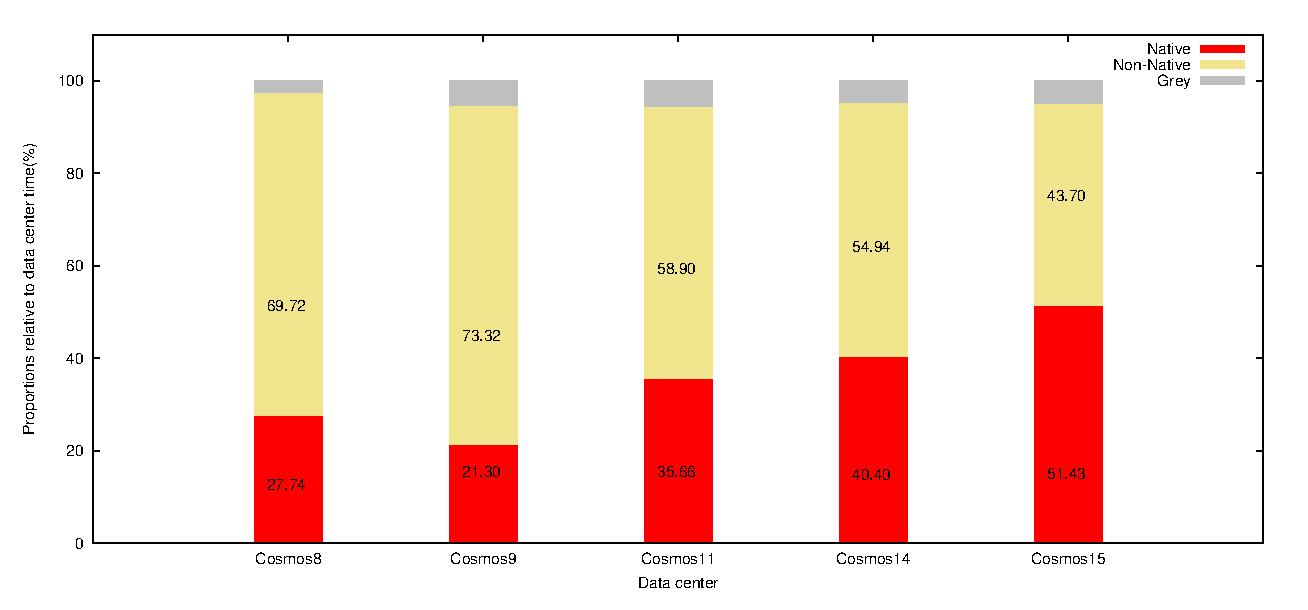
\includegraphics[scale = 0.7]{graphs/proportions}
\caption{Time spent in native vs. non-native vertices}
\end{figure*}

\subsection{Optimizable Job Stages}

This figure illustrates how much time is spent in job stages that we can optimize by inlining the user-written logic. X axis represents data center, Y axis represents precentage of time spent in inlineable job stages relative to total data center time and total time spent in non-native code.

\begin{figure}[ht]
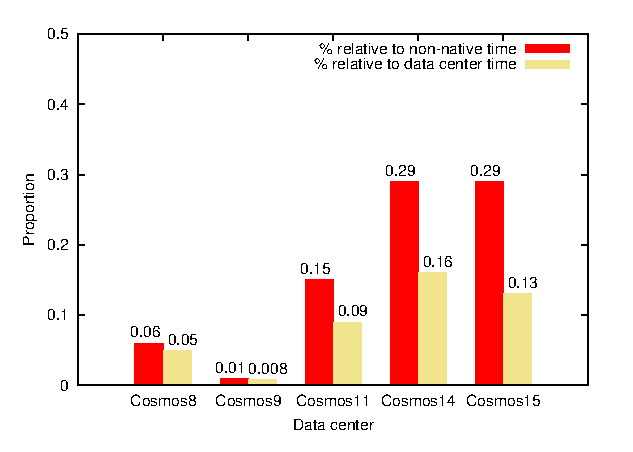
\includegraphics[scale=0.8]{graphs/optimizable}
\caption{Optimizable job vertices}
\end{figure}

\subsection{Potential for C++ Translation}

The following figure shows how much time can be affected by extending the list of functions that have C++ implementations. X axis represents data center, Y axis precentage of time spent in job stages that can be optimized, relative to total non-native and data center time.

\begin{figure}[ht]
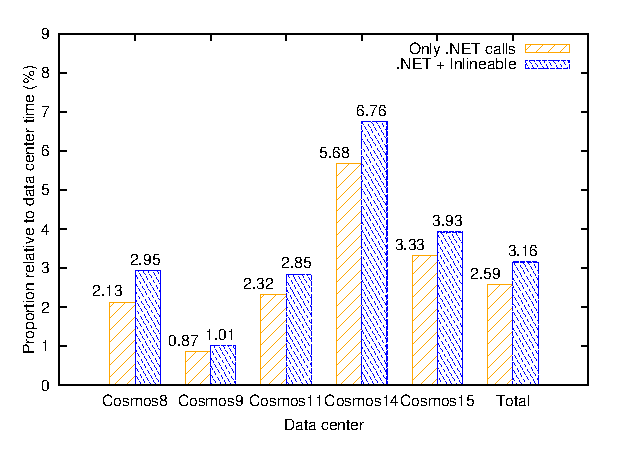
\includegraphics[scale=0.8]{graphs/potentiallyOptimizable}

\caption{Potentially optimizable job vertices}
\end{figure}

\subsubsection{Most Relevant .NET Framework Methods}

Ranking criteria: cost of job stage
\begin{table*}[ht]
\small
 \begin{tabular}{@{}llllp{3.5cm}@{}}

  Cosmos8 & Cosmos9 & Cosmos11 & Cosmos14 & Cosmos15 \\
 \midrule
System.Convert.ToInt64 & \textbf{System.String.Equals} & System.String.Replace & \textbf{System.DateTime.ToString} & \textbf{System.String.ToLower} \\
System.Int32.Parse & \textbf{System.String.ToLower} & \textbf{System.String.ToLower} & System.String.IndexOf & System.String.LastIndexOf \\
\textbf{System.String.ToLower} & System.Int32.Parse & System.String.ToUpper & System.DateTime.ToLocalTime & \textbf{System.DateTime.ToString}\\
\textbf{System.String.Concat} & System.String.Replace & \textbf{System.String.Concat} & \textbf{System.String.ToLower} & \textbf{System.String.Concat}\\
System.String.Replace & System.Convert.ToDateTime & System.String.Trim & System.String.ToUpper & System.Convert.ToUInt64 \\
System.Double.Parse & System.Regex.isMatch & System.Math.Max & System.Regex.IsMatch & System.Enumerable.SelectMany \\
System.Math.Round& System.DateTime.ToUniversalTime & \textbf{System.String.Equals} & \textbf{System.String.Equals} & System.Enumerable.Distinct \\
System.Char.NewArr & \textbf{System.String.Concat} & System.TimeSpan.Days & \textbf{System.String.Concat} & System.String.Format \\
System.String.ToUpper & System.TimeSpan.Days & \textbf{System.DateTime.ToString} & System.String.Trim & \textbf{System.String.Equals}\\
System.String.Upper & System.DateTime.Subtract & System.String.ToCharArray & System.String.Split & System.String.IndexOf \\

\midrule
1.27\%\footnote{proportion relative to data center time} & 0.63\% & 1.61\% & 5.15\% & 1.8\%\\
\midrule

\end{tabular}
 \label{tb:projects}
\caption{Most relevant .NET Framework methods per data center}
\end{table*}

The table below shows for every data center what are the most important .NET framework methods taking into account our ranking criteria...Furthermore, it illustrates how much time would be affected by providing C++ implementation of these methods, relative to total non-native time and total data center time.

\begin{figure}[ht]
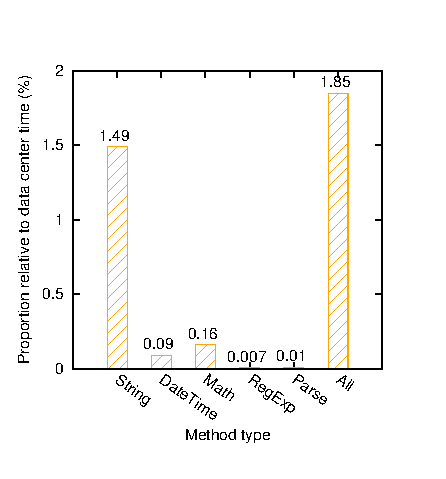
\includegraphics{graphs/methodTypes}
\caption{Relevance of .NET framework method types}
\label{fig:methodTypes}
\end{figure}









\section{Case Studies}
\label{sec:caseStudy}
In order to quantify the effects of optimizing the scripts, we performed a case study.
We say that a C\# method is {\em intrinsicable} if it is a .NET Framework method for which the SCOPE compiler has a semantically equivalent C++ function.
The jobs were chosen based on a static analysis that found {\em optimizable vertices}.
An optimizable vertex is one that is implemented in C\#, but the C\# code calls only intrinsicable methods or user-defined functions, {\em UDFs}, where the UDF, in turn, calls only intrinsicable methods, and does not call any other UDFs, i.e., our inlining depth is one.
We then manually looked at the top jobs from  a ranked list (by CPU time) of jobs containing an optimizable vertex.

Because the input data for each job is not available, we needed to contact the job owners and ask them to re-run the job with a manually-inlined version of their script.
We were able to have \casestudyjobs{} jobs re-run by their owners.
We roughly categorize the jobs by their total CPU time: short, medium, and long.

\subsection{Optimizations With Effects On Job Algebra}
As explained in Section~\ref{sec:intro}, the optimizer may choose to modify the job algebra given the new information available to it.
For example, predicates might be pushed deeper into the DAG which can result in dramatic data reduction.
However, none of the case studies ended up causing this kind of optimization.


\subsection{Optimizations Without Effects On Job Algebra}
Even if the physical plan does not change, the resulting program might be might more efficient if it avoids the native to managed transition.
For SCOPE, the set of intrinsics means that by lifting more non-relational code into the parts of the program where such things are visible to the optimizer, more code can be executed in C++ instead of in C\#.

\begin{figure*}[ht]
\begin{tabular}{c|c|c|c|c|c} 
\toprule
  {\em Job Name} & {\em C++ translation}&{\em Job Cost} & \multicolumn{2}{c}{\em CPU time} &  {\em Throughput } \\
  \cmidrule{4-5}  
  & & & {\em Vertex Change} & {\em Job Change} &  \\
  \midrule

A & yes & medium & 59.63\%  & 23.00\% & 30\% \\
B &yes & medium & no change & no change & no change\\
C & yes & low    & 41.98\%  & 25.00\% & 38\% \\
D & no & - & - & - & -\\
E & yes & high   & 7.22\%   & 4.79\% &  5\% \\
F & yes & low & no change & no change & 115\% \\

%For Jobs A and B the numbers are averages over the a one week period.
\end{tabular}
\caption{Summary of case studies. The reported changes are percent improvements in CPU time and throughput. \label{fig:caseStudySummary}}
\end{figure*}

In total, we looked at \casestudyjobs{} re-run jobs, summarized in Figure~\ref{fig:caseStudySummary}. 
For one job (D), the optimization did not trigger C++ translation of an inlined operator because the operator called to a non-intrinsicable method that we mistakenly thought was an intrinsic.
After fixing this problem, we used the correct set of intrinsics to obtain data presented in Section~\ref{sec:evaluation}.
\begin{figure}[ht]
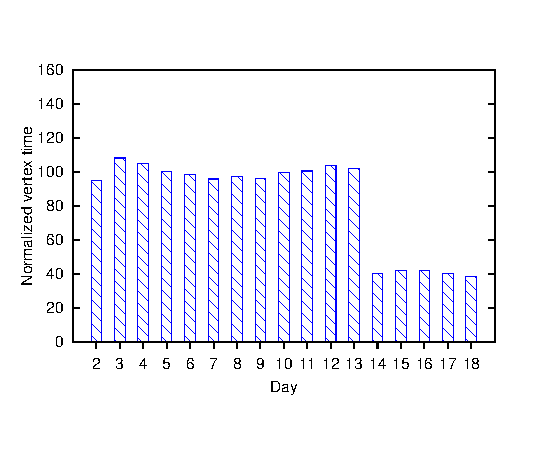
\includegraphics{graphs/normalizedTimesA}
\caption{Case Study A \label{fig:CaseStudyA}}
\end{figure}

\begin{figure}[ht]
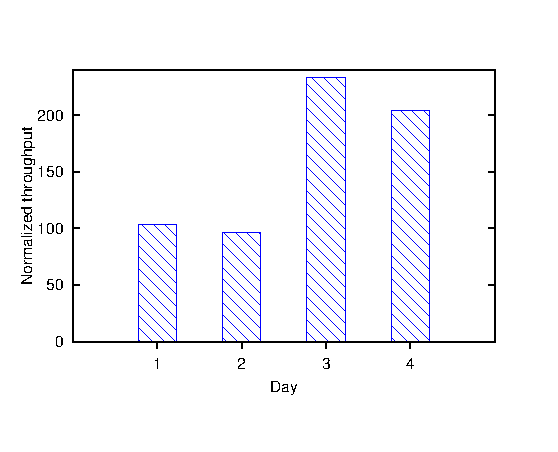
\includegraphics{graphs/throughtputF}
\caption{Case Study F \label{fig:CaseStudyF}}
\end{figure}


For jobs A and B, we were able to perfom the historical study over a period of 18 days. 
Both jobs are medium-expensive jobs, run daily and contain exactly one optimizable vertex due to a UDF. In both cases, inlining that UDF resulted in the entire vertex being executed in C++.
Figure~\ref{fig:CaseStudyA} shows the CPU time for an optimized vertex in Job A over an 18 day period, the last 5 of which were with the inlined UDF.
The values are normalized by the average of the unoptimized execution times; the optimized version saves approximately 60\% of the execution time.
However, the normalized vertex CPU time in Job B does not show any consistent improvement for the last five jobs.
Closer analysis of the vertex shows that the operator which had been in C\# accounted for a very tiny percentage of the execution time for the vertex.
This is consistent with our results for Job A, where the operator had essentially been 100\% of the execution time of the vertex.


We also optimized Job F, a very low cost job.
It only runs a few times a month, so we were able to obtain timing information for only a few executions.
The vertex containing the optimized operator accounted for over 99\% of the overall CPU time for the entire job.
We found the CPU time to be highly variable; perhaps this is because the job runs so quickly so it is more sensitive to the batch environment in which it runs.
However,  we found the throughput measurements to be consistent: the optimized version provided twice the throughput for the entire job (again, compared to the average of the unoptimized version).

Finally, for jobs C and E we were not able to perform the same kind of historical study: instead we have just one execution of the optimized scripts. 
For this execution we found improvements in both vertex and job CPU times.


% Job A  is guid 74a1edb8
% Job B is guid 9b432578
% Job C is guid 01e72a39 and vertex SV4_Extract
% Job D is guid 0414cd51
% Job E is guid f2bd0961 and SV1_Extract_Combine_Split
% Job F is guid ac127d4f

\section{Limitations And Threads to Validity}


\paragraph{Underapproximation of performance impact}
\paragraph{Assumptions for static analysis}
\paragraph{Challenges for implementing more intrinsics}


\section{Related Work}
\subsection{Query Optimizations}

....


\section{Future Work \label{sec:future}}

We plan to pursue several avenues in the near future.
First, we would like to do a broader set of experiments.
Even in our limited case studies we found that it is not always beneficial to
inline UDFs.
It would be necessary to have an analysis that can predict when to perform the optimization. 

Furthermore, we would like to explore ways to relax the restrictions on which methods we can inline.
In particular, user-defined operators (UDOs) consume an inordinate amount of time in each data center: being able to optimize them could provide a very large benefit.

Finally, exploiting other optimizations in the context of big data jobs at Microsoft is also left for future work.

\section{Conclusions}



\section*{Acknowledgements}
We want to especially thank the SCOPE team for answering our endless questions and also the product groups that helped us experiment with their scripts.

\bibliographystyle{ACM-Reference-Format}
\bibliography{references} 

\end{document}
